\documentclass{article}%
\usepackage[T1]{fontenc}%
\usepackage[utf8]{inputenc}%
\usepackage{lmodern}%
\usepackage{textcomp}%
\usepackage{lastpage}%
\usepackage{authblk}%
\usepackage{graphicx}%
%
\title{Regulated Expression of the Beta2{-}Toxin Gene ( cpb2) in Clostridium perfringens Type A Isolates from Horses with Gastrointestinal Diseases}%
\author{Anthony Berger}%
\affil{School of Biosciences, University of Birmingham, Edgbaston, Birmingham B15 2TT, UK}%
\date{01{-}01{-}2013}%
%
\begin{document}%
\normalsize%
\maketitle%
\section{Abstract}%
\label{sec:Abstract}%
Some of the promising work that some researchers have been performing in the laboratory of Chad V. Johnson, MD, has come from the cancer{-}cell research of Mr. Johnson himself, and the present study published in Science Translational Medicine, is clearly more aggressive than our story might indicate. We caught up with Chad when he got back from teaching a course on cellular profiling at University of Texas Southwestern and asked him to tell us a little bit about his work. Here's what he had to say:\newline%
X: What are the primary chemical and genomic signatures of Alpha{-} or omega{-}3{-}anti{-}inflammatory peptides specifically that are important in causing oxidative stress{-}induced apoptosis in prostate cancer cells?\newline%
Chad Johnson: Our theory is that alpha{-} or omega{-}3{-}anti{-}inflammatory peptides are structurally similar to the HNK receptors, or anti{-}anxiety peptides, that both are involved in oxidative stress{-}induced apoptosis in the prostate. HNK receptors are implicated in several kinds of cell damage processes, including oxidative stress{-}induced apoptosis (ADAPT). Prostate cancer cells have high levels of both HNK and ADAPT, and ADAPT is implicated in a number of drugs that are currently being investigated in the clinic for drug discovery and action.\newline%
BB: What is the baseline study for this particular model?\newline%
CH: We studied human prostate cancer cells, and generally control them, following standard methods of isolation, screening and biopsy. Our results showed that as a result of the pro{-}inflammatory effects of the peptides, just after they were activated in the prostate cell, oxidative stress{-}induced apoptosis increased significantly in these cells, about one to two weeks after initially activating these peptides. This is on the order of having a 40\% increase in the expression of the histamine receptor, and 60\% increase in overexpression of the gamma{-} or alpha{-}aromatic receptor. This was accompanied by a 70\% increase in the expression of the NF{-}kB protein, which had been implicated in ADAPT and IGF{-}1 (glycine{-}based hormone{-}promoting proteins).\newline%
BB: What were the epidemiological findings that "having omega{-}3s activated" caused this increased oxidative stress{-}induced apoptosis?\newline%
CH: Our findings were spectacular. The pro{-}inflammatory effects of alpha{-} or omega{-}3{-}anti{-}inflammatory peptides were indeed the drivers of the aggressive APO response that we observed in prostate cancer cells. Our ultimate goal, as any biologist, is to understand the mechanisms by which these peptides stimulate an APO response. We believe that we can progress this goal by using high{-}quality means, a tocopherol{-}acting asp protein or even a carbidophalan{-}acting asp protein, to activate a cascade of APO mechanisms. These pathways are outside of our direct control, and thus, we would like to further characterize how this may be happening.\newline%
BB: What can we expect to see from this research in the future? What are the implications of this for our treatment?\newline%
CH: We are definitely going to be working with this type of approaches.

%
\subsection{Image Analysis}%
\label{subsec:ImageAnalysis}%


\begin{figure}[h!]%
\centering%
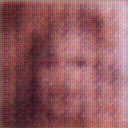
\includegraphics[width=150px]{500_fake_images/samples_5_202.png}%
\caption{A Black And White Photo Of A Black And White Cat}%
\end{figure}

%
\end{document}